\documentclass{report}

%Coloque as duas linhas abaixo no preâmbulo do arquivo.
\usepackage{tikz}
\usetikzlibrary{patterns}

\begin{document}

% % % % % % % % % % AQUI COMEÇA A FIGURA % % % % % % % % % %
\begin{figure}
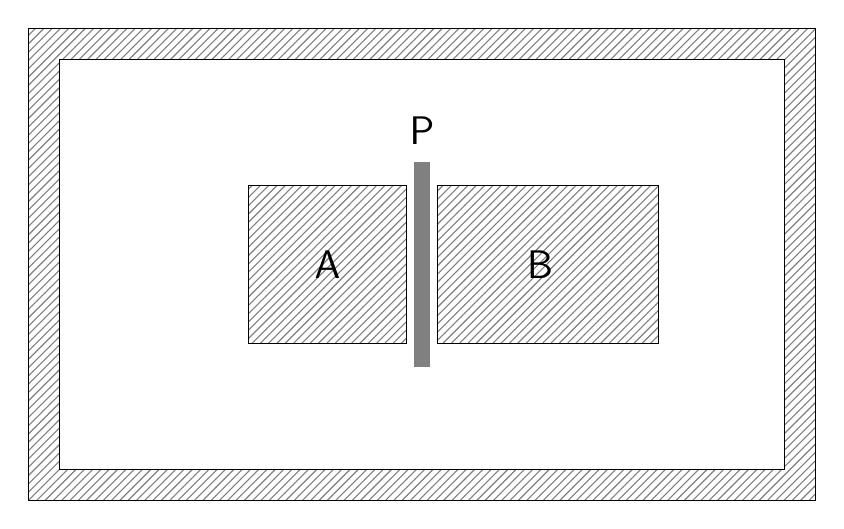
\begin{tikzpicture}[scale=1]
% Caixa maior
\draw[pattern=north east lines, pattern color=gray] (0,-1) rectangle (10,5);
\draw[fill=white] (0.4,-0.6) rectangle (9.6,4.6);

% Caixa A
\draw[pattern=north east lines, pattern color=gray] (2.8,1) rectangle (4.8,3);
\node at (3.8,2) {\textsf{\Large{A}}};

% Caixa B
\draw[pattern=north east lines, pattern color=gray] (5.2,1) rectangle (8,3);
\node at (6.5,2) {\textsf{\Large{B}}};

% Separação P
\draw[fill=gray,gray] (4.9,0.7) rectangle (5.1,3.3);
\node at (5,3.7) {\textsf{\Large{P}}};

% Grid para facilitar os cálculos
%\draw[help lines] (-1,-1) grid (11,6);	

\end{tikzpicture}
\caption{Esta é a legenda da figura.}
\end{figure}
% % % % % % % % % % AQUI TERMINA A FIGURA % % % % % % % % % %

\end{document}